\section{Evolutionary Exploration of Compiler Optimizations }


Lots of techniques (meta-heuristics, constraint programming, etc.) can be used to explore the large set of optimization combinations of modern compilers. 
In our approach, we study the use of the Novelty Search (NS) technique to identify the set of compiler optimization options that optimize non-functional properties of code.

\subsection{Novelty Search Adaptation}
%Optimization options are difficult and even impossible to be chosen by programmers or compiler users.
%Therefore, a tool to help users to choose the best set of options becomes necessary to achieve a compiler optimization with effectiveness.

In this work, we aim at providing a new alternative for choosing effective compiler optimization options compared to the state of the art approaches. 
In fact, since the search space of possible combinations is too large, we aim at using a new search-based technique called Novelty Search~\cite{lehman2008exploiting} to tackle this issue. 
The idea of this technique is to explore the search space of possible compiler flag options by considering sequences diversity as a single objective. 
Instead of having a fitness-based selection that maximizes one of the non-functional objectives, we select optimization sequences based on a novelty score showing how different they are compared to all other combinations evaluated so far. 
We claim that the search toward effective optimization sequences is not straightforward since the interactions between optimizations is too complex and difficult to define. 
For instance, in a previous work~\cite{chen2012deconstructing}, Chen et al. showed that handful optimizations may lead to higher performance than other techniques of iterative optimization. 
In fact, the fitness-based search may be trapped into some local optima that can not escape. 
This phenomenon is known as \textit{"diversity loss"}. For example, if the most effective optimization sequence that induces less execution time, lies far from the search space defined by the gradient of the fitness function, then some promising search areas may not be reached. 
The issue of premature convergence to local optima has been a common problem in evolutionary algorithms. 
Many methods are proposed to overcome this problem~\cite{banzhaf1996effect,gathercole1996adverse}. 
However, all these efforts use a fitness-based selection to guide the search. Considering diversity as the unique objective function to be optimized may be a key solution to this problem.
Therefore, during the evolutionary process, we select optimization sequences that remain in sparse regions of the search space in order to guide the search toward novelty. 
In the meanwhile, we choose to gather non-functional metrics of explored sequences such as memory consumption. 
We describe in more details the way we are collecting these non-functional metrics in section 4.

Generally, NS acts like GAs (Example of GA use in  \cite{cooper2002adaptive}). However, NS needs extra changes. First, a new novelty metric is required to replace the fitness function. Then, an archive must be added to the algorithm which is a kind of a database that remembers individuals that were highly novel when they were discovered in past generations. 
Algorithm~\ref{algo:search} describes the overall idea of our NS adaptation. The algorithm takes as input a source code program and a list of optimizations. We initialize first the novelty parameters and create a new archive with limit size L (line 1 \& 2). In this example, we gathered information about memory consumption. In line 3 \& 4, we compile and execute the input program without any optimization (O0). Then, we measure the resulting memory consumption. By doing so, we will be able to compare it to the memory consumption of new generated solutions. The best solution is the one that yields to the lowest memory consumption compared to O0 usage.
Before starting the evolutionary process, we generate an initial population with random sequences. Line 6-21 encode the main NS loop, which searches for the best sequence in terms of memory consumption. For each sequence in the population, we compile the input program, execute it and evaluate the solution by calculating the average distance from its k-nearest neighbors. Sequences that get a novelty metric higher than the novelty threshold T are added to archive. T defines the threshold for how novel a sequence has to be before it is added to the archive. In the meantime, we check if the optimization sequence yields to the lowest memory consumption so that, we can consider it as the best solution. Finally, genetic operators
(mutation and crossover) are applied afterwards to fulfill the next population. This process is iterated until reaching the maximum number of evaluations.


\begin{algorithm}
\algsetup{linenosize=\tiny}
  \footnotesize
  %footnotesize
	\caption{Novelty search algorithm for compiler optimizations exploration}
	\label{algo:search}
	\begin{algorithmic}[1]
	
		\REQUIRE Optimization options $\mathcal{O}$
		\REQUIRE Program $\mathcal{C}$
		\REQUIRE Novelty threshold $\mathcal{T}$
		\REQUIRE Limit $\mathcal{L}$
		\REQUIRE Nearest neighbors $\mathcal{K}$
		\REQUIRE Number of evaluations $\mathcal{N}$
		\ENSURE Best optimization sequence $best\_sequence$
		\STATE $initialize\_parameters(\mathcal{L},T,N,K)$
		\STATE $create\_archive(\mathcal{L})$
		\STATE 	$generated\_code \gets compile(\textit{"-O0"},\mathcal{C})$
		\STATE 	$minimum\_usage \gets execute(generated\_code)$
		\STATE $population \gets random\_sequences(\mathcal{O})$
		\REPEAT
		\FOR{$sequence \in population$}   
		\STATE 	$generated\_code \gets compile(sequence,\mathcal{C})$
		\STATE 	$memory\_usage \gets execute(generated\_code)$
		\STATE	$novelty\_metric(sequence) \gets distFromKnearest(archive,population,\mathcal{K})$
		\IF{$novelty\_metric > \mathcal{T}$}
		\STATE	$archive \gets archive \cup sequence$
		\ENDIF
		
			\IF{$memory\_usage < minimum\_usage$}
			\STATE	$best\_sequence \gets sequence$
			\STATE	$minimum\_usage \gets memory\_usage$
			\ENDIF
			
		\ENDFOR
		\STATE		$new\_population \gets generate\_new\_population(population)$
		\STATE		$generation \gets generation + 1$
		\UNTIL{generation = N}
		\RETURN $best\_sequence$
	\end{algorithmic}
\end{algorithm}


\subsubsection{Optimization Sequence Representation}
For our case study, a candidate solution represents all compiler switches that are used in the 4 standard optimization levels (O1, O2, O3 and Ofast). Thereby, we represent this solution as a vector where each dimension is a compiler flag. 
The variables that represent compiler options are represented as genes in a chromosome. 
Thus, a solution represents the CFLAGS value used by GCC to compile programs.
A solution has always the same size which corresponds to the total number of involved flags. 
However, during the evolutionary process, these flags are turned on or off depending on the mutation and crossover operators (see example in figure 2). As well, we keep the same order of invoking compiler flags since that does not affect the optimization process and it is handled internally by GCC.
\begin{figure}[h]
	\centering
	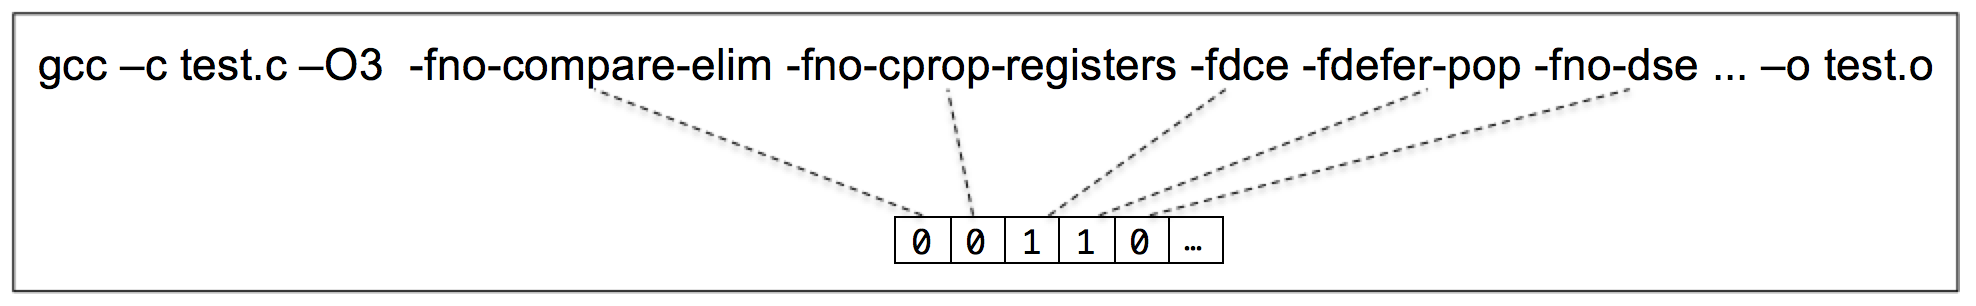
\includegraphics[width=1\hsize]{Ressources/individual.png}
	\caption{Solution representation}
\end{figure}

\subsubsection{Novelty Metric}
The Novelty metric expresses the sparseness of an input optimization sequence. It measures its distance to all other sequences in the current population and to all sequences that were discovered in the past (\ie, sequences in the archive). 
We can quantify the sparseness of a solution as the average distance to the k-nearest neighbors. 
If the average distance to a given point's nearest neighbors is large then it belongs to a sparse area and will get a high novelty score. 
Otherwise, if the average distance is small so it belongs certainly to a dense region then it will get a low novelty score. 
The distance between two sequences is computed as the total number of symmetric differences among optimization options. Formally, we define this distance as follows :
\begin{equation}
distance(S1,S2)=\left | S1 \bigtriangleup S2 \right |
\end{equation}
where $S1$ et $S2$ are two selected optimization sequences (solutions). In this equation, we calculate the cardinality of the symmetric difference between two sequences. This distance is 0 if two optimization sequences are similar and higher than 0 if there is at least one optimization difference. The maximum distance is equal to the total number of input flags.

To measure the sparseness of a solution, we use the previously defined distance to compute the average distance of a sequence to its k-nearest neighbors. In this context, we define the novelty metric of a particular solution as follows:
\begin{equation}
NM(S) = \frac{1}{k} \sum_{i=1}^{k} distance(S,\mu _{i})
\end{equation}
where $\mu _{i}$ is the $i^{th}$ nearest neighbor of the solution S within the population and the archive of novel individuals. 

\subsection{Novelty Search For Multi-objective Optimization}
A multi-objective approach provides a trade-off between two objectives where the developers can select their desired solution from the Pareto-optimal front. The idea of this approach is to use multi-objective algorithms to find trade-offs between non-functional properties of generated code such as \textit{$<$ExecutionTime--MemoryUsage$>$}. The correlations we are trying to investigate are more related to the trade-offs between resource consumption and execution time.
  
For instance, NS can be easily adapted to multi-objective problems. In this adaptation, the SBSE formulation remains the same as described in Algorithm 1. However, in order to evaluate the new discovered solutions, we have to consider two main objectives and add the non-dominated solutions to the Pareto non-dominated set. We apply the Pareto dominance relation to find solutions that are not Pareto dominated by any other solution discovered so far, like in NSGA-II~\cite{lokuciejewski2010multi, deb2002fast}. Then, this Pareto non-dominated set is returned as the result. The metric used to evaluate one solution compared to previously discovered ones is called Hypervolume (HV)~\cite{deb2001multi}.
There is typically more than one optimal solution at the end of NS. The size of the final Pareto set yielded is bounded by the size of the initial population chosen.
